\renewcommand\thechapter{c2.15a}
\lab{Faraday's Law}\label{lab:faraday}

\section*{About this lab}

\covid\ 
It is intended to be used around the 15th week in Physics 222.

\apparatus
\equip{banana plug cables (8, soldered by the student)}
\equip{USB oscilloscope (Hantek)}
\equip{two oscilloscope probes with BNC connectors}
\equip{assorted capacitors capacitors, 10-100 nF}
\equip{alligator clips (5)}
\equip{two hand-made coils}


\begin{goals}

\item[] Test Faraday's law.
\end{goals}

\introduction

Physicists hate complication, and when physicist Mi\-ch\-a\-el
Faraday was first learning physics in the early 19th
century, an embarrassingly complex aspect of the science was
the multiplicity of types of forces. Friction, normal
forces, gravity, electric forces, magnetic forces, surface
tension --- the list went on and on. Today, 200 years later,
ask a physicist to enumerate the fundamental forces of
nature and the most likely response will be ``four: gravity,
electromagnetism, the strong nuclear force and the weak
nuclear force.'' Part of the simplification came from the
study of matter at the atomic level, which showed that
apparently unrelated forces such as friction, normal forces,
and surface tension were all manifestations of electrical
forces among atoms. The other big simplification came from
Faraday's experimental work showing that electric and
magnetic forces were intimately related in previously
unexpected ways, so intimately related in fact that we now
refer to the two sets of force-phenomena under a single
term, ``electromagnetism.''

Even before Faraday, Oersted had shown that there was at
least some relationship between electric and magnetic
forces. An electrical current creates a magnetic field, and
magnetic fields exert forces on an electrical current. In
other words, electric forces are forces of charges acting on
charges, and magnetic forces are forces of moving charges on
moving charges. (Even the magnetic field of a bar magnet is
due to currents, the currents created by the orbiting
electrons in its atoms.)

Faraday took Oersted's work a step further, and showed that
the relationship between electricity and magnetism was even
deeper. He showed that a changing electric field produces a
magnetic field, and a changing magnetic field produces an
electric field. Faraday's law,
\begin{equation*}
      \int \vc{E}\cdot\bell  =  -\der\Phi_B/\der t  
\end{equation*}
relates the integral of the electric field around a
closed loop to the rate of change of the magnetic flux
through the loop. It forms the basis for such technologies
as the transformer, the electric guitar, the amplifier, and
generator, and the electric motor.

\section*{Preparation}

Work out the theoretical equation as described in the analysis section.

\section*{Setup}

This lab is a quantitative test of Faraday's
law. 

For the first time in this lab course, you will be using both channels
of the oscilloscope.
Put the oscilloscope's probe (the one you've been using all semester)
on x1.
The second oscilloscope probe that comes with the scope does not have
a x1/x10 switch. In the software, check the box to turn on channel 2,
which will show up as a blue trace.


\subsection*{Simplified conceptual setup}

The first figure shows a simplified conceptual schematic for the lab.
We would use a sine wave generator to provide an AC voltage, which
would drive an AC current $\tilde{I}_1$  through the primary coil. This current
is measured by an AC ammeter. The current can be related to the magnetic
field created by the primary coil. Because the current oscillates,
the magnetic field oscillates as well.

\fig{em-faraday-conceptual-covid}

This changing magnetic field induces an electric field, which has
a certain value of $\int \vc{E}\cdot\bell$ as we integrate around
all the loops of the secondary coil. This quantity has units of
volts, and is often referred to as an emf (standing for ``electromotive
force,'' which is not a very accurate term). It is measured as an AC
voltage $\tilde{V}_2$ by the AC voltmeter. Faraday's law can be
used to make a prediction of the form $\tilde{V}_2=(\text{const.})\tilde{I}_1$.
We measure $\tilde{I}_1$ and $\tilde{V}_2$, and determine whether the constant
factor is as predicted by Faraday's law.

\subsection*{Real setup}

The realistic circuit is shown in the second figure. The oscilloscope is
a voltmeter, not an ammeter, so we measure a voltage and a voltage, not
a current and a voltage. This type of application is an example of why the oscilloscope has two channels,
each of which gives an independent measurement of a voltage as a function of time.
Conceptually, each of these channels is an input with two terminals, so there are four
connections from the circuit to the scope's inputs. But in reality, both channels
have one terminal tied to the same USB ground, so to keep the diagram simple I've
just shown those connections as connections to ground. You do really have to connect
the primary circuit to the ground clip of channel 1's probe, and on channel 2 you
do really have to complete the circuit by connecting to the ground clip.

\fig{em-faraday-covid}

The scope's calibration output is a square-wave generator, not a sine-wave
generator. As in lab \ref{lab:ac-circuits}, this can be Fourier analyzed
as
$\raisebox{-.2\height}{\includegraphics{../figs/eqn-wave1}}
+\frac{1}{3}\raisebox{-.2\height}{\includegraphics{../figs/eqn-wave3}}
+\frac{1}{5}\raisebox{-.2\height}{\includegraphics{../figs/eqn-wave5}}
+\ldots$ There is somewhat of a tendency for the higher-frequency sine
waves to get filtered out because of the primary coil's higher impedance
at high frequencies, but actually this filtering is not very strong because
most of the impedance comes from the internal resistor inside the scope,
which you investigated in lab \ref{lab:covid-oscilloscope}. (This is the
resistor shown in the schematic.) It's nicer to do this lab with a simple
sine wave, so we add a capacitor as shown in order to filter out the
high frequencies better. This is fairly simple to understand qualitatively.
In the limit of very high frequencies, the capacitor's impedance goes to
zero. This then forms a short across the inductor, putting the inductor
out of action.

In this setup, we don't actually measure the current $\tilde{I}_1$ through
the primary coil but rather the voltage $\tilde{V}_1$ across it. However,
these two quantities are related to each other. This relationship does
have the inductance $L_1$ in it, but you've already determined that inductance
in lab \ref{lab:ac-circuits}. (If your two coils are different from each other,
then you will want to use the one whose inductance is known as your primary coil.)

The geometry you use for the coils may depend on exactly how they're constructed.
For example, you could nest the secondary inside the primary, if it fits
and if there's a hole down the central axis of the primary. Mine didn't
fit that way, so I ended up with the geometry shown below in cross-section. To make the
calculations practical, you will need to make an approximation by
calculating the flux through the secondary coil as if the field created by
the primary coil was uniform and parallel to the axis, and had the value
calculated at a point (dot) at the center of the secondary coil. This is
discussed further in the analysis section. By making this approximation,
you will find a prediction based on Faraday's law of the form $\tilde{V}_2=\alpha \tilde{V}_1$,
where $\alpha$ is a unitless constant. We'll ignore the sign of $\alpha$ because
it depends on how you hook up each coil, and it can be hard to tell on these hand-made
coils which way the wires turn, especially if you end up using duct tape to hold the
wires in place, as I did.

\fig{em-faraday-geometry}

\observations

To start with,  just set up the primary circuit, and leave an open circuit
in place of the capacitor, so there is no extra filtering. I ended up using
a frequency of 50 kHz for the square wave, but you may end up doing something
slightly different. On channel 1 of the scope, you should see a series of
alternating shark-fin pulses. This should be the response of an RL circuit
to a square wave, which is basically a series of exponential curves, each
of which should have the time constant $L/R$. In reality, I found poor
agreement of this time constant (a factor of four discrepancy) with $L/R$ when I used the previously
measured values of $L$ and $R$. This may have to do with nonideal behavior of
the coil at high frequencies, such as stray capacitance.

It's actually not terribly
important for our purposes to be able to predict or explain the waveform seen on channel
1 in quantitative detail. Our goal is just to get it to be a reasonably clean signal
that looks more or less like a sine wave. Try to make this happen by putting in
different values for the filtering capacitor and possibly by playing with the
frequency of the calibration output. I ended up using a capacitance of 33 nF,
which with my coil gave reasonably sinusoidal-looking voltage with an amplitude
$|\tilde{V}_1|$ of about half a volt.

If you now connect channel 2 to the secondary coil, you should see a waveform
that mimics the one on channel 1, but with a different amplitude. For my coils,
$\alpha$ was about 0.1, so the signal on channel 2 was quite a bit weaker, and I
had to adjust the vertical scale to make it visible.

You should be able to make the signal on channel 2 get weaker by moving the
coils farther apart, and you should be able to flip the sign of $\alpha$
by either turning one coil around physically or reversing the connections
onto it.

Measure $|\tilde{V}_1|$, $|\tilde{V}_2|$, and all the geometrical dimensions.;

\analysis

Compare your observations quantitatively with Faraday's law.
The primary isn't very long, so the approximate expression for the
interior field of a long solenoid isn't very accurate here. To correct
for that, multiply the expression for the field by the correction
factor $\zeta = (\cos\theta_1-\cos\theta_2)/2$,
(\emph{Fields and Circuits}, ch.~11, problem 13), where
$\theta_1$ and $\theta_2$ are angles between the axis and the lines connecting
the point of interest to the edges of the solenoid's mouths.

This analysis is horrible to do and to read if you do it all numerically.
From Faraday's law, you should be able to
express $\alpha$ symbolically in terms of the following
symbols:
\begin{align*}
 k  &= \text{Columb constant} \\
 c  &= \text{speed of light} \\
 N_1  &= \text{number of turns in the primary coil} \\
 N_2  &= \text{number of turns in the secondary coil} \\
 \omega  &= \text{frequency} \\
 A  &= \text{area of the secondary coil} \\
 L  &= \text{inductance of the primary coil} \\
 \ell_1  &= \text{length of the primary coil} \\
 \zeta  &= \text{correction factor for the magnetic field}.
\end{align*}
Check that the units work. You should find that the frequency cancels out.
Only plug in numbers at the end.

